\chapter{評価}
\par
行動情報と発話情報の両方を反映した心的状態の推定が有効であることを示すため,信念および欲求の推定において,MIoMと単一情報による心的状態推定システムUnimodal Inference of Mind(UIoM)を比較する.行動情報と発話情報には,本研究で作成したデータセットを利用する.本データセットの詳細は後述する.

\section{実験設定}

\begin{figure}[htbp]
  \begin{center}
    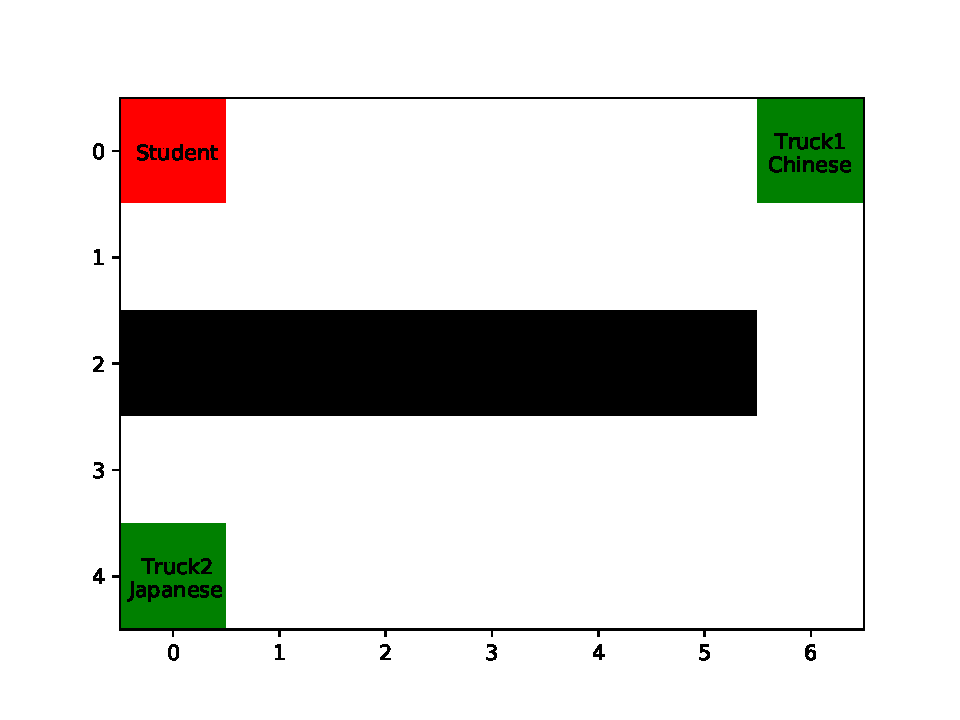
\includegraphics[]{./figure.pdf}
    \caption{本実験における環境}
    \label{fig:ex_env}
  \end{center}
\end{figure}

\par
学生がアシストロボットとともに屋台で食事を買うシーンを想定する.図\ref{fig:ex_env}に本実験における環境の一例を示す.7$\times$5マスで表現される環境中に屋台を開くスペースが2箇所存在し,それぞれのスペースに日本食の屋台,イタリア料理の屋台,中華料理の屋台のいずれかが出店する.環境中の学生は移動し,対話システムと対話をしながら食事を購入する屋台を決める状況を考える.学生は,日本食の屋台,イタリア料理の屋台,中華料理の屋台の3種類のうち2種類が出店することは知っているが,どの屋台が出店しているかは知らないため,環境中を移動しアシストロボットと対話しながら食事を買う屋台を選ぶ.学生の行動$a_t$は上,下,左,右の4方向への移動とし,発話$u_t$はアシストロボットから提示される食事に関する質問に対する学生の応答とする.信念$b_t$は,どの屋台が出店していると考えているか,欲求$d$は学生が3種類の屋台をどの順に好むかを表す.


\section{実験手順}

\par
本実験には,本研究で作成したデータセットを利用した.本データセットには,屋台の組み合わせを表す環境設定と,その環境設定で考えられる学生の行動,アシストロボットからの質問,学生の応答が含まれる.屋台の組み合わせは日本食の屋台,イタリア料理の屋台,中華料理の屋台の2つの組み合わせとする6通り,学生の行動は上,下,左,右の4方向への移動,アシストロボットからの質問は表\ref{tab:question}に記載される4通り,学生の応答は表\ref{tab:answer}に記載される8通りである.30人の実験参加者に,本データセットで指定された環境設定と行動およびアシストロボットからの質問と学生の応答を提示し,環境中の学生の信念と欲求をそれぞれ7段階で推定させた.またMIoMと,行動情報と発話情報の一方のみを基に心的状態を推定するUnimodal Inference of Mind(UIoM)により信念と欲求の推定を行った.MIoM(action + utterance),行動情報のみを基に心的状態を推定するUIoM(action),発話情報のみを基に心的状態を推定するUIoM(utterance)の3つのシステムによって,環境中の学生の信念と欲求をそれぞれ7段階で推定した.実験参加者によって得られた推定結果とMIoMおよびUIoM によって得られた推定結果を比較し相関係数を算出した.

\begin{table}[htb]
  \begin{center}
  \caption{アシストロボットからの質問}
  \label{tab:question}
  \begin{tabular}{c} \hline
    質問内容\\\hline
    魚料理と野菜料理どちらを食べたいですか\\
    パスタと米ではどちらを食べたいですか\\
    あっさりしたものと,こってりしたものどちらを食べたいですか\\
    辛いものと酸っぱいものではどちらを食べたいですか\\\hline
  \end{tabular}
\end{center}
\end{table}

\begin{table}[htb]
  \begin{center}
  \caption{学生の応答}
  \label{tab:answer}
  \begin{tabular}{cc} \hline
    \multicolumn{2}{c}{応答内容}\\\hline
     fish & vegetable \\
     pasta & rice \\
     plain & oily \\
     spicy & sour \\\hline
  \end{tabular}
\end{center}
\end{table}


\section{実験結果}

\begin{table}[htb]
  \begin{center}
  \caption{人間による推定と推定モデルの相関}
  \label{tab:cof}
  \begin{tabular}{lcc} \hline
    \multirow{2}{*}{モデル}&\multicolumn{2}{c}{相関}\\\cline{2-3}
    & \hspace{10pt} 信念 \hspace{10pt} & \hspace{10pt} 欲求 \hspace{10pt} \\ \hline
    UIoM(action)&0.124&0.419\\
    UIoM(utterance)&0.216&0.494\\
    MIoM(action + utterance)&\bf0.244&\bf0.549 \\\hline
  \end{tabular}
\end{center}
\end{table}


\par
表\ref{tab:cof}に,実験参加者による信念と欲求の推定結果とUIoM(action), UIoM(utterance)およびMIoMによる信念と欲求の推定結果との間の相関係数を示す.

\par
表\ref{tab:cof}より,MIoMは信念と欲求の推定の両方においてUIoM(action)およびUIoM(utterance)よりも強い相関を示した.また,いずれの推定システムにおいても欲求推定の相関が信念推定の相関よりも強いことがわかった.
